\section{Методи локалізації людини та рухомих об'єктів}
\subsection{Локалізація рухомих об'єктів}

Розглянемо теоретичне підґрунтя методів, які використовуються в даній роботі для
локалізації рухомих об'єктів, а саме задачу пошуку мінімального розрізу графа
та її розв'язок за допомогою алгоритму Бойкова-Колмогорова.

\subsubsection{Задача знаходження мінімального розрізу графа}

Задачу знаходження мінімального розрізу та еквівалентна їй задачу пошуку максимального потоку
можна описати на прикладі системи трубопроводу.
Є мережа труб, кожна з яких має свою пропускну здатність і напрям.
У даній мережі є джерело (початок мережі) та стік (кінець мережі).
Головна задача ~---~ знайти максимальний потік води,
який може пройти з джерела у стік.

Якщо дану концепцію перекласти на мову
математики, то мережею труб є орієнтований граф $G$ (рис. \ref{fig:graph_example})
з множинами вузлів $T$ та множиною направлених ребер $\tau$.
В ньому є джерело $s \in T$, стік $e \in T$, пропускні здатності $c_{tt'} \ge 0$
та потоки $f_{tt'} \in \mathbb{R}$.
Також позначимо множини вихідних $N_t = \{t^{'}: tt^{'} \in \tau \}$
та вхідних $P_t = \{t: tt' \in \tau \}$ ребер для кожної вершини $t$.
\begin{definition}
    Максимальний потік ~---~  це найбільша величина потоку, який
    можна пропустити через джерело з метою найефективнішого  використання мережі.
\end{definition}

\begin{definition}
    Мінімальним розріз ~---~ це множина тих ребер, які стали насиченими після знаходження максимального
    потоку. Мінімальний розріз розділяє множину ребер на дві множини.
\end{definition}
\begin{figure}[H]
    \centering
    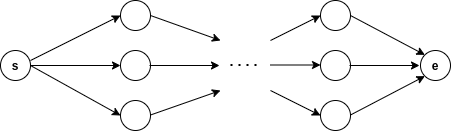
\includegraphics[width=0.5\textwidth]{images/graph_example}
    \caption{Приклад графу
        \label{fig:graph_example}
    }
\end{figure}

Сформулюємо задачу максимального потоку
\begin{equation*}
    \sum_{t \in N_s} f_{st} \rightarrow \max_{f: \tau \rightarrow R }
\end{equation*}
з обмеженнями
\begin{equation*}
    \begin{gathered}
        \begin{cases}
            f_{tt^{'}} \leq  c_{tt^{'}},                                   & \forall tt^{'}  \in \tau ,         \\
            \sum_{p \in P_t} f_{pt} - \sum_{t^{'} \in N_t} f_{tt^{'}} = 0, & \forall t \in T \setminus \{s,e\}, \\
            \sum f_{tt^{'}} \geq 0,                                        & \forall tt^{'}  \in \tau.
        \end{cases}
    \end{gathered}
\end{equation*}
Це означає, що
\begin{enumerate}
    \item потік має не перевищувати пропускну здатність для всіх ребер;
    \item сума потоків, що входять у вузол не повинна змінитись на виході;
    \item потік завжди додатній.
\end{enumerate}

Як вже було зазначено,
задача пошуку максимального потоку є еквівалентною до задачі пошуку мінімального розрізу.
Даний висновок отримується з Max-Flow Min-Cut теореми \cite{bib:ford_fulkerson, bib:edmods_karp}.

Наведемо алгоритм знаходження максимального потоку Форда-Фалкерсона (алгоритм \ref{al:ford_fulkerson_mas_flow}).

\begin{algorithm}[H]
    \caption{Алгоритм (метод) Форда-Фалкерсона пошуку максимального потоку}
    \label{al:ford_fulkerson_mas_flow}
    \begin{algorithmic}
        \State \textbf{Вхід:} граф $G$ з об'єктами $ t \in T $ і ребрами $tt^{'} \in \tau$.
        \State \textbf{Вихід:} $ F_{maxflow} $ - значення максимального потоку.
        \State \textbf{Ініціалізація:} $ F_{maxflow} = 0, f_{tt^{'}}^{0} = 0 \quad \forall tt^{'}  \in \tau $.
        \State \textbf{Поки існує шлях з $s$ в $e$ повторюємо кроки 1,2:}
        \State \textbf{Крок 1:} Знаходимо шлях від $s$ до $e$ (пошуком в ширину чи в глибину).
        \State Відвідуємо $ t^{'}$ із $t $ якщо:
        \State \qquad 1. $ f_{tt^{'}} \neq c_{tt^{'}} $
        \State \qquad 2. $ \nexists p_{t^{'}}^{i} \implies p_{t^{'}}^{i} = t $ (запам'ятали вершину)
        \State \qquad 3. $ t^{'} \neq s $
        \State \textbf{Крок 2:} Проходимо по заданому шляху:
        \State \qquad 1. Знаходимо $ \vartriangle f^{i} = \min_{tt^{'} \in \{шлях із s в e \}} $
        \State \qquad 2. Змінюємо потік: $ f_{tt^{'}}^{i+1} = f_{tt^{'}}^{i} + \vartriangle f^{i} $
        \State \qquad 3. Оновлюємо $ F_{maxflow}: F_{maxflow}^{i+1} = F_{maxflow}^{i} + \vartriangle f^{i} $
    \end{algorithmic}

    Знайшовши максимальний потік, можемо знайти і мінімальний розріз: \\
    $\forall t \in T$ знаходимо $\theta_{t} \in \{0,1\}$
    \begin{algorithmic}
        \State \textbf{Крок 3}: Запускаємо пошук в ширину або глибину вже з оновленим графом.
        \State \qquad Якщо $c_{tt^{'}} \geqslant f_{tt^{'}}$ та $c_{tt^{'}} \geqslant 0$
        $\implies \theta_{t^{'}} = 1 $, інакше $\theta_{t^{'}} = 0 $
    \end{algorithmic}
\end{algorithm}

У 2004 році Юрій Бойков та Володимир Колмогоров запропонували свій підхід \cite{bib:boykov_kolmogorov}
для пошуку мінімального розрізу на графі.
Запропонована ідея методу полягає у нарощенні потоку у шляхах з джерела та стоку.
Будується два дерева $S$ та $T$, коренями яких є $s$ та $t$ відповідно.
Вершини загально діляться на ті що в $S$, $T$ та
вільні. Кожне дерево має активні та внутрішні вершини.
Алгоритм Бойкова-Колмогорова (надалі Б-К алгоритм) складається зі стадій росту,
доповнення та всиновлення.
Коротко розглянемо кожну з них.
\begin{enumerate}
    \item \textbf{Стадія Росту.}
          Проводимо одночасний ріст дерев з вершин $s$ та $e$, знаходимо активні
          вершини і додаємо їх як вершини, що відвідали. Після такого сканування вершини
          стають внутрішніми. Цей процес продовжується поки не залишиться не активної вершини.
    \item \textbf{Стадія Доповнення.}
          На цій стадії потік вздовж шляху, що був знайдений на попередньому етапі,
          доповнюється залишковою пропускною здатністю (англ. bottleneck). Якщо ребра дерева стають
          насиченими (пропускна здатність дорівнює потоку), то найвіддаленіші вершини від коренів дерев стають
          сиротами, тобто, якщо вершини $t$ та $t^{'}$ додаються в множину $S$
          і ребро $(t,t^{'})$ є насиченим, тоді $t^{'}$ називається $S$-сиротою.
          Аналогічно, якщо $t$ та $t^{'}$ знаходяться в дереві $T$, то  $t$ ~---~ $T$-сирота.
          Якщо ребро знаходиться в bottleneck ($t$ в $S$, $t^{'}$ в $T$, ребро $(t,t^{'})$
          насичене) відповідно немає ніяких сиріт. Всі сироти потрапляють у множину сирот.
    \item \textbf{Стадія Всиновлення.}
          На даному етапі ми проходимось по кожній сироті в множині сирот для кожного дерева.
          Нехай $t^{'}$ є $S$-сиротою. Знаходимо всі такі $t$  в $S$, що
          $(t, t^{'}) \in E$. Для кожного такого $t$ перевіряємо, чи шлях з $t$ в $s$ містить сирот,
          включаючи $t$. Якщо сирот не знайшли, то $t$ ~---~ батько  $t^{'}$.
          Якщо не вдається знайти батька, ми позначаємо вершину $t^{'}$ як вільну, а всіх
          дітей $t^{'}$ сиротами. Після цього ми оброблюємо залишкові ребра $(t,t^{'})$ і для кожного $t$ в $S$ позначаємо
          $t$ активною.
\end{enumerate}

\begin{figure}[h]
    \centering
    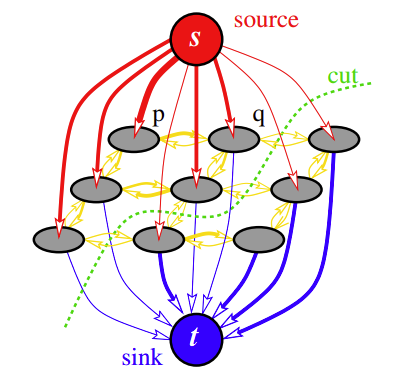
\includegraphics[width=0.3\textwidth]{images/graph_cut}
    \caption{Приклад графу-решітки з мінімальним розрізом \cite{bib:boykov_kolmogorov}
        \label{fig:graph_lattice}
    }
\end{figure}
Найбільшою перевагою даного алгоритму є те, що на практиці він працює дуже швидко на графах-решітках
(рис. \ref{fig:graph_lattice}).
Оскільки саме таку структуру ми використовуємо в алгоритмі Б-К для отримання маски рухомих
об'єктів, це дає змогу оброблювати кадри відео досить швидко.
